\documentclass[12]{beamer}

\usepackage[russian]{babel}
\usepackage{tikz}


\usetheme[progressbar=frametitle]{metropolis}
\setbeamertemplate{frame numbering}[fraction]
\usefonttheme{metropolis}
\setbeamercolor{background canvas}{bg=white}


\title{Семинар 3}
\subtitle{Копрпускулярно-волновой дуализм. Соотношение неопределенностей}
\author{}
\date{\today}
\institute {\large 
\textbf{Ключевые слова}: \\[6pt] 
соотношение неопределённостей
\\[6pt] 
\textbf{Задачи}: \\[6pt] 
2.15 2.43 2.31
}


\begin{document}
\metroset{block=fill}
\maketitle


\begin{frame}[t]{Корпускулярно-волновой дуализм}
\begin{block}{Вопрос}
Если волна ведет себя как частица, может ли и частица вести себя как волна?
\end{block}
Это работало для волн:
\begin{equation*}
    p = \dfrac{E}{c}=\dfrac{\hbar \omega}{c} = \hbar k = \dfrac{h}{\lambda}
\end{equation*}
Попробуем заставить это же работать для частиц, например элетрон, разогнанного в поле с напряжением $U=100$ В
\begin{equation*}
    \lambda = \dfrac{h}{m_eV} = \dfrac{h}{\sqrt{2m_eeU}} \approx \dfrac{10^{-34}}{\sqrt{10^{-31}\cdot10^{-19}\cdot10^{2}}} \text{ м} \approx 10^{-10} \text{ м}
\end{equation*}

\end{frame}

\begin{frame}[t]{Корпускулярно-волновой дуализм}
\begin{block}{Вопрос}
Если волна ведет себя как частица, может ли и частица вести себя как волна?
\end{block}
Это работало для волн:
\begin{equation*}
    p = \dfrac{E}{c}=\dfrac{\hbar \omega}{c} = \hbar k = \dfrac{h}{\lambda}
\end{equation*}
Попробуем заставить это же работать для частиц, например элетрон, разогнанного в поле с напряжением $U=100$ В
\begin{equation*}
    \lambda = \dfrac{h}{m_eV} = \dfrac{h}{\sqrt{2m_eeU}} \approx \dfrac{10^{-34}}{\sqrt{10^{-31}\cdot10^{-19}\cdot10^{2}}} \text{ м} \approx 10^{-10} \text{ м}
\end{equation*}

\end{frame}




\begin{frame}[t]{Опыт Дэввисона-Джермера}
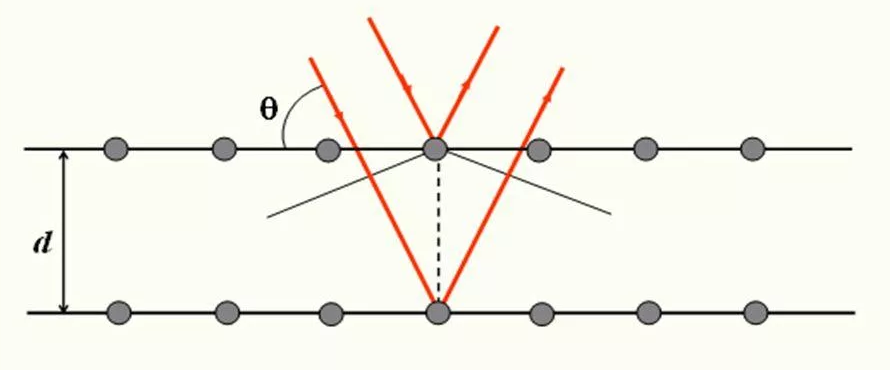
\includegraphics[width=\textwidth]{Seminar_03/pics/pres_pic_01.PNG}
Условие Брэгга-Вульфа
\begin{equation*}
    2d\sin{\theta} = n\lambda
\end{equation*}

\end{frame}

\begin{frame}[t]{Интерференция электронов}
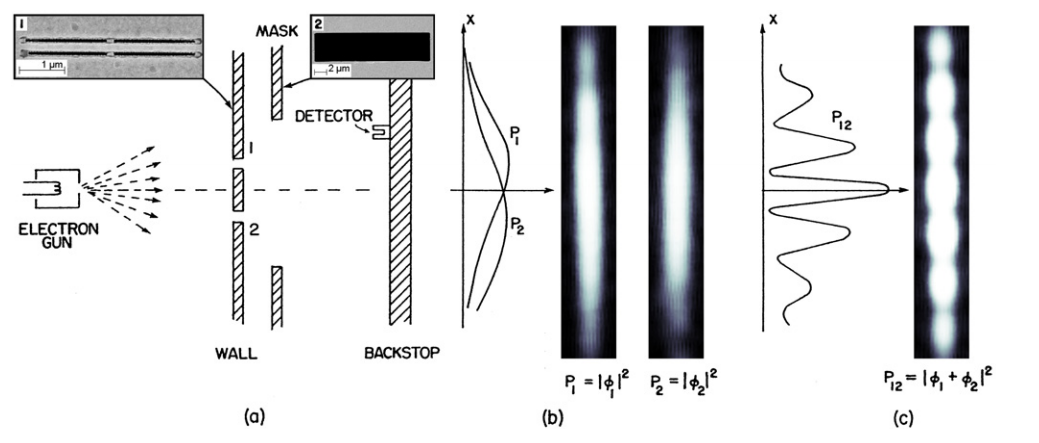
\includegraphics[width=\textwidth]{Seminar_03/pics/pres_pic_02.PNG}
Схема установки из эксперимента Баха 2013 года\\
\begin{block}{Волна де Бройля}
\begin{equation*}
    \psi = \psi_0 \exp{\left[i\left(kx - \omega t \right)\right]} =\psi_0 \exp{\left[\dfrac{i}{\hbar}\left(px - Et \right)\right]}
\end{equation*}
\end{block}
\end{frame}

\begin{frame}[t]{Измерение. Соотношение неопределенностей}
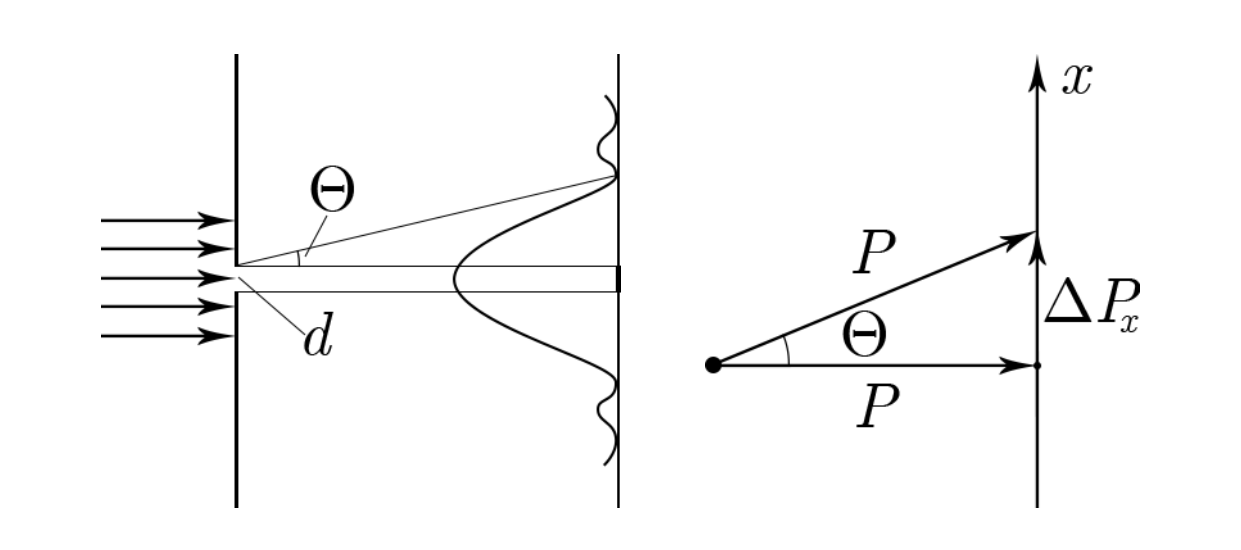
\includegraphics[width=0.7\textwidth,keepaspectratio]{Seminar_03/pics/pic_02.png}
$\lambda = h/p; \sin{\theta} = \lambda/d; \sin{\theta} = \Delta p / p$ \\$d\Delta p = h$.
\begin{block}{Соотношение неопределённостей}
\begin{gather*}
    \Delta p_x \Delta x \sim h \text{ или более точно } \sigma^2_p \sigma^2_x \ge \dfrac{\hbar^2}{4}\\
    \Delta E \Delta t \sim h
\end{gather*}
\end{block}
\end{frame}


\begin{frame}{Задача Задача 2.15}\scriptsize
\only<1>{
\begin{block}{Условие}
Чтобы получить пучок нейтронов обладающих заданной энергией $E = 1$ эВ используют брэгговское отражение первого порядка от кристалла LiF, для которого расстояние между плоскостями решетки $d = 2.32$ \AA. На кристалл падает пучок нейтронов с различными энергиями. Оценить разброс нейтронов по энергиям в отраженном пучке, если его угловая ширина $\Delta \varphi = 0.1$ градуса. Какую толщину кристалла $D$ следует выбирать в этом эксперименте?
\end{block}

}
\only<2>{
\begin{block}{Решение}\scriptsize
Условие Брэгга-Вульфа и  масштаб бедствия по углам отклонения:
\begin{gather*}
    \sin{\varphi} = \dfrac{\lambda}{2d}\\
    \lambda = \dfrac{h}{p} = \dfrac{h}{\sqrt{2mE}} \approx 0.287 \text{ \AA;}
    \sin{\varphi} \approx \varphi \approx 0.06
\end{gather*}
Из закономерности: $\lambda \sim \varphi  \sim E^{-1/2} $:
\begin{equation*}
    \dfrac{\Delta \lambda}{\lambda} = \dfrac{\Delta \varphi}{\varphi} = \dfrac{\Delta E}{2E}
\end{equation*}
Выражаем отсюда $\Delta E = 2E \dfrac{\Delta \varphi}{\varphi} \approx 0.58$ эВ\\
Вопрос с толщиной. Дифракционная решетка с разрешающей способностью:
\begin{gather*}
    \dfrac{\Delta \lambda}{\lambda} \le R = mN = 1\cdot \dfrac{D}{d}
\end{gather*}
окончательно $D = \dfrac{\lambda}{2\Delta \varphi} = 82 \text{ \AA}$
\end{block}
}
\end{frame}

\begin{frame}{Задача 2.43 }\scriptsize
\only<1>{\begin{block}{Условие}
Оценить на основании соотношения неопределенностей радиус атома водорода в основном состоянии и энергию связи электрона в том же состоянии. Определить на основании таких же оценок размер двухатомной молекулы и энергию её основного состояния,рассматривая молекулу как одномерный гармонический осциллятор с собственной частотой $\omega_0$ и приведенной массой $\mu$
\end{block}}
\only<2>{\begin{block}{Решение. Атом водорода}
 Неопределенности : $\Delta x \sim r; \Delta p \sim p \Rightarrow p\cdot r = \hbar $. \\
 Полная энергия электрона в атоме водорода:
\begin{gather*}
    E = \dfrac{p^2}{2m} - \dfrac{e^2}{r} = \dfrac{\hbar^2}{2mr^2} - \dfrac{e^2}{r}
\end{gather*}
Атом находится в основном состоянии, значит, в состоянии с минимальной энергией. Найдем минимум через производную энергии по времени. 
\begin{gather*}
    \dfrac{dE}{dt} = -\dfrac{\hbar^22r}{2mr^4} + \dfrac{e^2}{r^2} = 0 \Rightarrow к = \dfrac{\hbar^2}{me^2}=0.53 \text{ \AA}
\end{gather*}
Тогда энергия основного состояния:
\begin{gather*}
     E = \dfrac{\hbar^2}{2mr^2} - \dfrac{e^2}{r} = -\dfrac{me^4}{2\hbar^2} = -13.6\text{ эВ}
\end{gather*}
Что интересно, эта оценка дает точно совпадающий с теорией Бора результат.
\end{block}}

\only<3>{\begin{block}{Решение. Осциллятор}
Неопределенности : $\Delta x \sim x; \Delta p \sim p $\\
Полная энергия для такой молекулы, с учетом соотношения в форме Вейля:
\begin{gather*}
     E = \dfrac{p^2}{2\mu} + \dfrac{kx^2}{2} = \dfrac{\hbar^2}{8\mu x^2} + \dfrac{\mu \omega_0^2 x^2}{2}
\end{gather*}
Аналогично первой части найдем минимум энергии:
\begin{gather*}
    \dfrac{dE}{dx^2} = -\dfrac{\hbar^4}{8\mu x^4} + \dfrac{\mu \omega_0^2}{2} = 0 \Rightarrow x^2 = \dfrac{\hbar}{2\mu\omega_0} \Rightarrow E = \dfrac{\hbar\omega_0}{2}
\end{gather*}
Этот результат оказывается также точно совпадает со строгим решением задачи о нулевом уровне энергии квантового гармонического осциллятора.
\end{block}}
\end{frame}

\begin{frame}{Задача 2.31}\scriptsize
\begin{block}{Условие}
Предполагая, что ядерные силы между нуклонами обусловлены обменом квантами ядерного поля -- виртуальными пионами, оценить радиус $\Delta r$ действия ядерных сил, если известно, что энергия покоя пионов $m_{\pi}c^2 \approx 140$ МэВ.
\end{block}
\begin{block}{Решение}
Вот тут нам и пригодиться соотношение неопределенностей энергия-время. 
\begin{gather*}
    R \le c\Delta t = c\dfrac{h}{\Delta E} = c\dfrac{h}{m_{\pi}c^2}\approx 2\cdot 10^{-13} \text{ см}
\end{gather*}
\end{block}
\end{frame}



\begin{frame}[t]{Комментарии к задачам из задания}\scriptsize
\begin{itemize}
\item Нулевки. В первой просто подставить в формулы, вторая по сути решена в 2.43
\item Задача 2.10. Решена в задачнике
\item Задача 2.15. Решена
\item Задача 2.26. Задачка ультра релятивистская, так что надо использовать формулу для полной энергии именно как корень, а дальше все получится
\item Задача 2.30. Часть решения я демонстрировал в теоретической части, а часть это просто оптика
\item Задача 2.38. Задача подозрительно напоминает часть 1 из 2.43
\item Задача 2.44. Решена в задачнике
\end{itemize}
\end{frame}

\end{document}